\chapter{Introduction}

\section{Speech Synthesis}

Speech is most important medium of conveying opinions and expressing feelings and thoughts.
Human convert their thoughts into speech by using words, phrases and sentences in order to communicate with each other \cite{mumtaz2016break}. 
Speech is produced when air is exhaled by the lungs and vibrations are produced by air, these vibrations got a 
proper waveform shape by glottal cords and vocal tract. Text to Speech synthesis is the process of conversion of raw text into 
speech signals. It works by concatenation of small segments of recorded speech called phonemes \cite{khilari2015review}. Speech data is obtained by first recording natural speech by using some type of recording systems and then converted to digital form. The digital data is sampled and stored in computer, after that passed back to analog signals and converted back to speech \cite{greene1986perception}. 

Text to speech systems are becomming important as they can be used in machine to effectively transmit
information to human using artificial speech as information exchange through computers has become the integral part of new
era. Partially blinded or fully blinded people usually suffer while using computer technology when there is no assistant or
computer is not enough interactive. Due to which text to speech systems are becoming necessity of modern life. These
systems increase the degree to which blind people can interact with sighted people \cite{klatt1987review} and could boost up
their hope to survive in this world gracefully \cite{aida2010main}. Many applications of speech synthesis are emerging such as 
machines that read for blinds, aids for handicaps, computers that interact with user through speech. 
For all these applications a text to speech that convert text to speech are used \cite{klatt1982klattalk}.

The TTS system comprises of two main stages. One is called Natural language Processing (NLP) and
other is called Speech Synthesis (SS). This is shown in figure \ref{fig:TTS Block Diagram}.

\begin{figure}[hp]
  \centering
  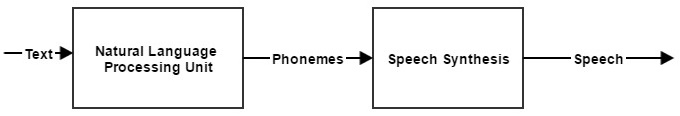
\includegraphics[width=\linewidth]{images/tts_bd.jpg}
  \caption{TTS Block Diagram}
  \label{fig:TTS Block Diagram}
\end{figure}

In NLP unit, text is first converted into string of letters and then word boundaries are marked by
tokenizer. This is called normalization of text. Normalized data is then converted into phonetic strings
with the help of letter to sound rules after which Syllabifier marks syllable boundaries. Sound change
rules are applied on the syllabified data. Language modeling techniques are also applied for finding
context in which a specific word is used. As human has tendency to recognize basic rules for his native
language, it is easy to judge context of a word in a sentence and what should be correct pronunciation of
that word with respect to its context. For example, it can be guessed easily that \enquote{\texturdu{پل}} in a sentence is used
for \texturdu{پل} (moment) or \texturdu{پل} (bridge) for any native speaker of Urdu. But for computer, we need to mark context of each word according to data. 
Last stage of NLP is stress intonation marker which adds stress and intonation to the text. Speech Synthesis unit converts symbolic information
received from NLP unit into audible speech with the help of different Digital Signal Processing
techniques. The quality of speech synthesis system is detected by naturalness and intelligibility of the speech.

In digital world, there are some people who can read and understand different languages and some
who can’t understand languages except their own languages. Speech to text conversion system can
also provide a facility to exchange information between people speaking different languages \cite{khilari2015review}. 
TTS systems are also needed to reduce the extinction of
minority languages. As minority languages of the world are facing challenge of extinction
considerable efforts are going on from last few years for their survival. Fon language is spoken in
Republic of Benin and some other regions of Africa and it is also facing challenge of extinction \cite{dagba2014text}. 
The Xitsonga is spoken in more than three African countries.
TTS system of such languages will help lot of people of different literacy level \cite{baloyi2012text}.
Urdu is national language of Pakistan and it is spoken by more than 100 million people across the world \cite{top_30_languages}.
A Text-to-Speech (TTS) system for Urdu will be very helping for visually impaired, handicapped and illiterate people.

For human, the task of speech synthesis is not difficult one as they have basic knowledge of their
language but for computer some
other method has to be implemented for this task. When we talk about TTS systems speech types
and procedure for synthesis, strategies or modules used to develop systems etc. are important to
consider. Different types of speech exist such as isolated word (process single word at a time),
connected words (isolated words but separated with least gap), continuous speech (permit client
to talk while computer is processing content) and spontaneous speech (deals with variety of words
that are used rarely) as well as two types of speaker model were presented independent and
dependent of clients or speaker specifications. Vocabulary is also characterized according to size
such as small vocabulary, medium vocabulary, large vocabulary, very large vocabulary and out-of-vocabulary.
Below are the major speech generation techniques.

\section{Types of Speech Synthesis}
For the process of speech synthesis, three types of techniques are used.

\subsection{Formant Synthesis}
In Formant Synthesis, speech waveform is generated using concatenation of sine wave with the help of some algorithms to model a source of sound \cite{format_synthesis}. All speech parameters are changed periodically in order to get speech waveform. Some set of rules are also used to generate speech due to which this technique is also called rule based speech synthesis. But it is very difficult to accurately describe the process of speech generation in set of rules therefor the speech generated by this technique is not very natural but intelligible.
\subsection{Concatenative Synthesis}
In concatenative synthesis small units are selected from carrier sentences which then join to form
speech of complete sentence. These small units are called phonemes. These are the units which
collectively describe correct pronunciation of a word. This process is easy as compared to previous one
as number of such phonemes is limited for any language. For English, there are 44 such phonemes.
Similarly in Urdu, there are 44 consonants, 8 long vowels, 7 long nasal vowels, 3 short vowels and many
diphthongs \cite{saleem2002urdu}. This reduce distortion but it can decrease the naturalness.
That’s why the derived synthetic speech may not resemble the donor speaker in training database \cite{huang1996whistler}.

\subsection{Statistical Parametric Speech Synthesis}
Statistical parametric speech synthesis is another approach which uses parameters to describe
speech. In this technique, model is learned from speech data. This technique works better than
concatenative technique \cite{merritt2013investigating}. 

\section{Quality of Speech Synthesis System}
Intelligibility and naturalness is the measure of quality of the synthesized speech \cite{swetha2013text}. 
There is lots of experimentation over naturalness of voice as a result of TTS
systems. In today’s world, different segments are recorded and then concatenated for completing a
message. A collection of speech words is collected and maintained in database by using a reader
who reads large series of text. In these kind of systems, to maintain the consistency the speaker
speaks in a single style and keep in mind the distance from microphone and other factors to avoid
the inconsistency. This type of TTS system is not required at all as the need is to have a system
which can be expressive and convey message with proper expressions and styles. Work is
performed to build a system that can convey the message according to the needs of the users. A
single style of communication can lead towards wrong messages and can cause other problems of
understandings. For example, it is not appropriate to convey a good news and bad news in a same
style and manner. Similarly, it is not acceptable to ask a question in neutral way of communication \cite{eide2004corpus}.
Multiple techniques like linear regression and neural networks were applied
to get the results with improvements. Concatenation techniques are applied to get fully
expressive and stylish messages for end users. By using concatenation technique, users can
customize, add styles and expression through provided Speech Synthesis Markup Language (SSML) \cite{eide2004corpus}. 
Timing of events in speech is also important as timing of events in
speech signals are affected by some contextual factors like phone identity factors. These factors
make it difficult to control timing of events \cite{tokuda2000speech}. There are some approaches which have been proposed
to control timing of events like linear regression \cite{kaiki1992linguistic} and tree regression \cite{riley1992tree}. 
A new technique is proposed in \cite{tokuda2000speech} where timing of events is
controlled by multi-dimensional Gaussian distribution based Hidden Markov model.
\section{Architecture}
Text to speech is a way of communication and transferring information using words and styles of
speaking \cite{eide2004corpus}. It has two processes which are text processing and speech
generation. In text processing given input text is processed so that to get appropriate chain of
phonemic units. Speech generator takes these units as inputs and convert them into synthetic
speech by selection of a unit from large corpus TTS system for small database is easier to
implement but not in good quality \cite{black2007statistical, zen2007hmm, raj2007text}.
Different researchers and developers used different strategies and architecture to develop TTS system. In \cite{kabir2002natural}, raw text is converted into intelligible speech signals by following two sub processes called High-level synthesis and Low-level synthesis. High-level
synthesis converts text into phonetic strings and Low-level synthesis converts these strings into
speech signals \cite{kabir2002natural}. In \cite{hussain2005phonological}, TTS system is divided in three modules.

\begin{enumerate}
  \item Natural language Processing
  \item Text Parameterization
  \item Speech Synthesis
\end{enumerate}

Natural Language processing unit converts text into phonetic strings. The second and
third stages use these phonetic strings and convert them into speech signals. This is shown in figure \ref{fig:Architecture of TTS}.

\begin{figure}
  \centering
  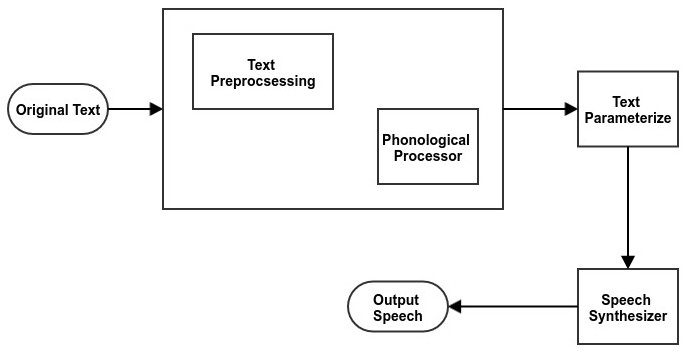
\includegraphics[width=\linewidth, height=7cm,keepaspectratio]{images/tts_block_dg.jpg}
  \caption{Architecture of TTS}
  \label{fig:Architecture of TTS}
\end{figure}

\\
In \cite{liberman1992text}, TTS system is implemented by following four modules in
sequence.

\begin{enumerate}
  \item Text Analysis
  \item Word Pronunciation
  \item Phonetic Interpretation
  \item Speech Signal Generation
\end{enumerate}

In text analysis, the input text is segmented into sentences and later on dividied into words.
These words are then categorized according to their syntactic and contextual meaning. The
numbers and abbreviations are also processed in this step. In word pronunciation process, words
are represented by respective phonetic notations by using word pronunciation dictionary. In
phonetic interpretation the duration of phonetic segments, pitch, accents are assigned. Signal
generation component of TTS system takes output from all above processes and generate a signal
of speech using a function. In \cite{urdu_text_preprocessing}, text-to-Speech system is divided in
two parts. One is called Natural Language Processing unit and other is called Speech Synthesis
unit. Natural Language Processing unit preprocess text and converts it into phonetic strings. These
phonetic strings are then marked by stress marker and passed to speech synthesis unit which
converts it into speech signals.